\documentclass[article]{jss}

%% -- LaTeX packages and custom commands ---------------------------------------

%% recommended packages
\usepackage{thumbpdf,lmodern}

%% additional packages
\usepackage{amssymb,amsmath}

%% new custom commands
\newcommand{\class}[1]{`\code{#1}'}
\newcommand{\fct}[1]{\code{#1()}}

%% For Sweave-based articles about R packages:
%% need no \usepackage{Sweave}



%% -- Article metainformation (author, title, ...) -----------------------------

%% - \author{} with primary affiliation
%% - \Plainauthor{} without affiliations
%% - Separate authors by \And or \AND (in \author) or by comma (in \Plainauthor).
%% - \AND starts a new line, \And does not.
\author{Lennart Oelschl\"ager \\Bielefeld University \And Timo Adam \\University of St Andrews\And Rouven Michels \\Bielefeld University}
\Plainauthor{Lennart Oelschl\"ager, Timo Adam, Rouven Michels}

%% - \title{} in title case
%% - \Plaintitle{} without LaTeX markup (if any)
%% - \Shorttitle{} with LaTeX markup (if any), used as running title
\title{\pkg{fHMM}: Hidden Markov Models for Financial Time Series in \proglang{R}}
\Plaintitle{fHMM: Hidden Markov Models for Financial Time Series in R}
\Shorttitle{fHMM}

%% - \Abstract{} almost as usual
\Abstract{
Hidden Markov models constitute a popular class of statistical models for time series that are driven by hidden states. In finance, these hidden states can often be linked to market regimes such as bearish and bullish markets or recessions and periods of economics growths, to name but a few examples. Hidden Markov models account for these state-switching patterns by... In this paper, we introduce the \proglang{R} package \pkg{fHMM} that provides various tools for modeling financial time series using hidden Markov models. Its key features include...
}

%% - \Keywords{} with LaTeX markup, at least one required
%% - \Plainkeywords{} without LaTeX markup (if necessary)
%% - Should be comma-separated and in sentence case.
\Keywords{decoding market behavior, hidden Markov models, time series modeling, \proglang{R}}
\Plainkeywords{decoding market behavior, hidden Markov models, time series modeling, R}

%% - \Address{} of at least one author
%% - May contain multiple affiliations for each author
%%   (in extra lines, separated by \emph{and}\\).
%% - May contain multiple authors for the same affiliation
%%   (in the same first line, separated by comma).
\Address{
  Lennart Oelschl\"ager\\
  Department of Business Administration and Economics\\
  Bielefeld University\\
  Postfach 10 01 31\\
  E-mail: \email{lennart.oelschlaeger@uni-bielefeld.de}
}

\begin{document}
\Sconcordance{concordance:fhmm_oelschlaeger_adam_michels.tex:fhmm_oelschlaeger_adam_michels.Rnw:%
1 16 1 1 5 110 1 1 2 4 0 1 2 51 1}

%% I have no idea what this does. Maybe we need this in the future.
%% \SweaveOpts{concordance=TRUE}

%% -- Introduction -------------------------------------------------------------

%% - In principle "as usual".
%% - But should typically have some discussion of both _software_ and _methods_.
%% - Use \proglang{}, \pkg{}, \fct{} and \code{} markup throughout the manuscript.
%% - If such markup is in (sub)section titles, a plain text version has to be
%%   added as well.
%% - All software mentioned should be properly \cite-d.
%% - All abbreviations should be introduced.
%% - Unless the expansions of abbreviations are proper names (like "Journal
%%   of Statistical Software" above) they should be in sentence case (like
%%   "generalized linear models" below).

\section{Introduction}
\label{sec:intro} %% Timo 

%% Earning money with stock trading is simple: one only needs to buy and sell stocks at the right moment. In general, stock traders seek to invest at the beginning of upward trends (hereon termed as bullish markets) and repel their stocks just in time before the prices fall again (hereon termed as bearish markets). As stock prices depend on a variety of environmental factors \cite{hum09}, \cite{coh13}, chance certainly plays a fundamental role in hitting those exact moments. However, investigating market behavior can lead to a better understanding of how trends alternate and thereby increases the chance of making profitable investment decisions. 

%% Intro to HMMs
In recent years, hidden Markov models (HMMs) have emerged as a popular tool for modeling time series that are subject to state-switching over time \citep{zuc16}. In their basic form, HMMs comprise an observed state-dependent process that is driven by a hidden state process, the latter of which is typically modeled using a discrete-time, finite-state Markov chain. In financial applications, the states of the underlying Markov chain can often be linked to market regimes such as bearish and bullish markets or recessions and periods of economics growths: when the market is in a calm state, then the observations follow some distribution, whereas when the market is in a nervous state, then another distribution is active to generate the observations. By their dependence structure, HMMs naturally account for such state-switching patterns and thus allow us to infer hidden market regimes and their dynamics from financial time series.

%% Literature review
Over the last decades, HMMs have been applied to various financial problems, including modeling business cycles \cite{gre00}, deriving stylized facts of stock returns \cite{bul06, nys15a}, and modeling energy prices conditional on market regimes \cite{lan18, ada22}, to name but a few examples.
More recently, \cite{lih17} used HMMs to identify different volatility levels in the Standard and Poor's 500 index, aiming at providing evidence for the conjecture that returns exhibit negative correlation with volatility. \cite{ngu18}, to give another example, used HMMs to predict monthly closing prices to derive an optimal trading strategy, which was shown to outperform the conventional buy-and-hold strategy. Further financial applications include HMMs for asset allocation and portfolio optimization \citep{bul11, nys15a, nys18}. All these examples demonstrate that HMMs constitute a versatile class of time series models that naturally accounts for the state-switching patterns that are often found in financial time series.

%% Intro to the package
The \pkg{fHMM} package aims at making HMMs accessible to users interested in modeling financial time series. Its functionality can be classified into functions for data preparation, model estimation, and model evaluation, which is illustrated in Figure \ref{fig:flowchart}. Functions for data preparation include an interface to Yahoo Finance... The model is estimated in a maximum likelihood framework, where the likelihood is evaluated using the forward algorithm, which is implemented in C++. Functions for model evaluation include...
%% The following flowchart visualizes their dependencies:
It also implements hierarchical HMMs; an extension of basic HMMs proposed in \cite{oel21} that improves the model's capability of distinguishing between short- and long-term trends and allows us to model data collected at different time scales. interpret market dynamics at multiple time scales. 

\begin{figure}
  \centering
  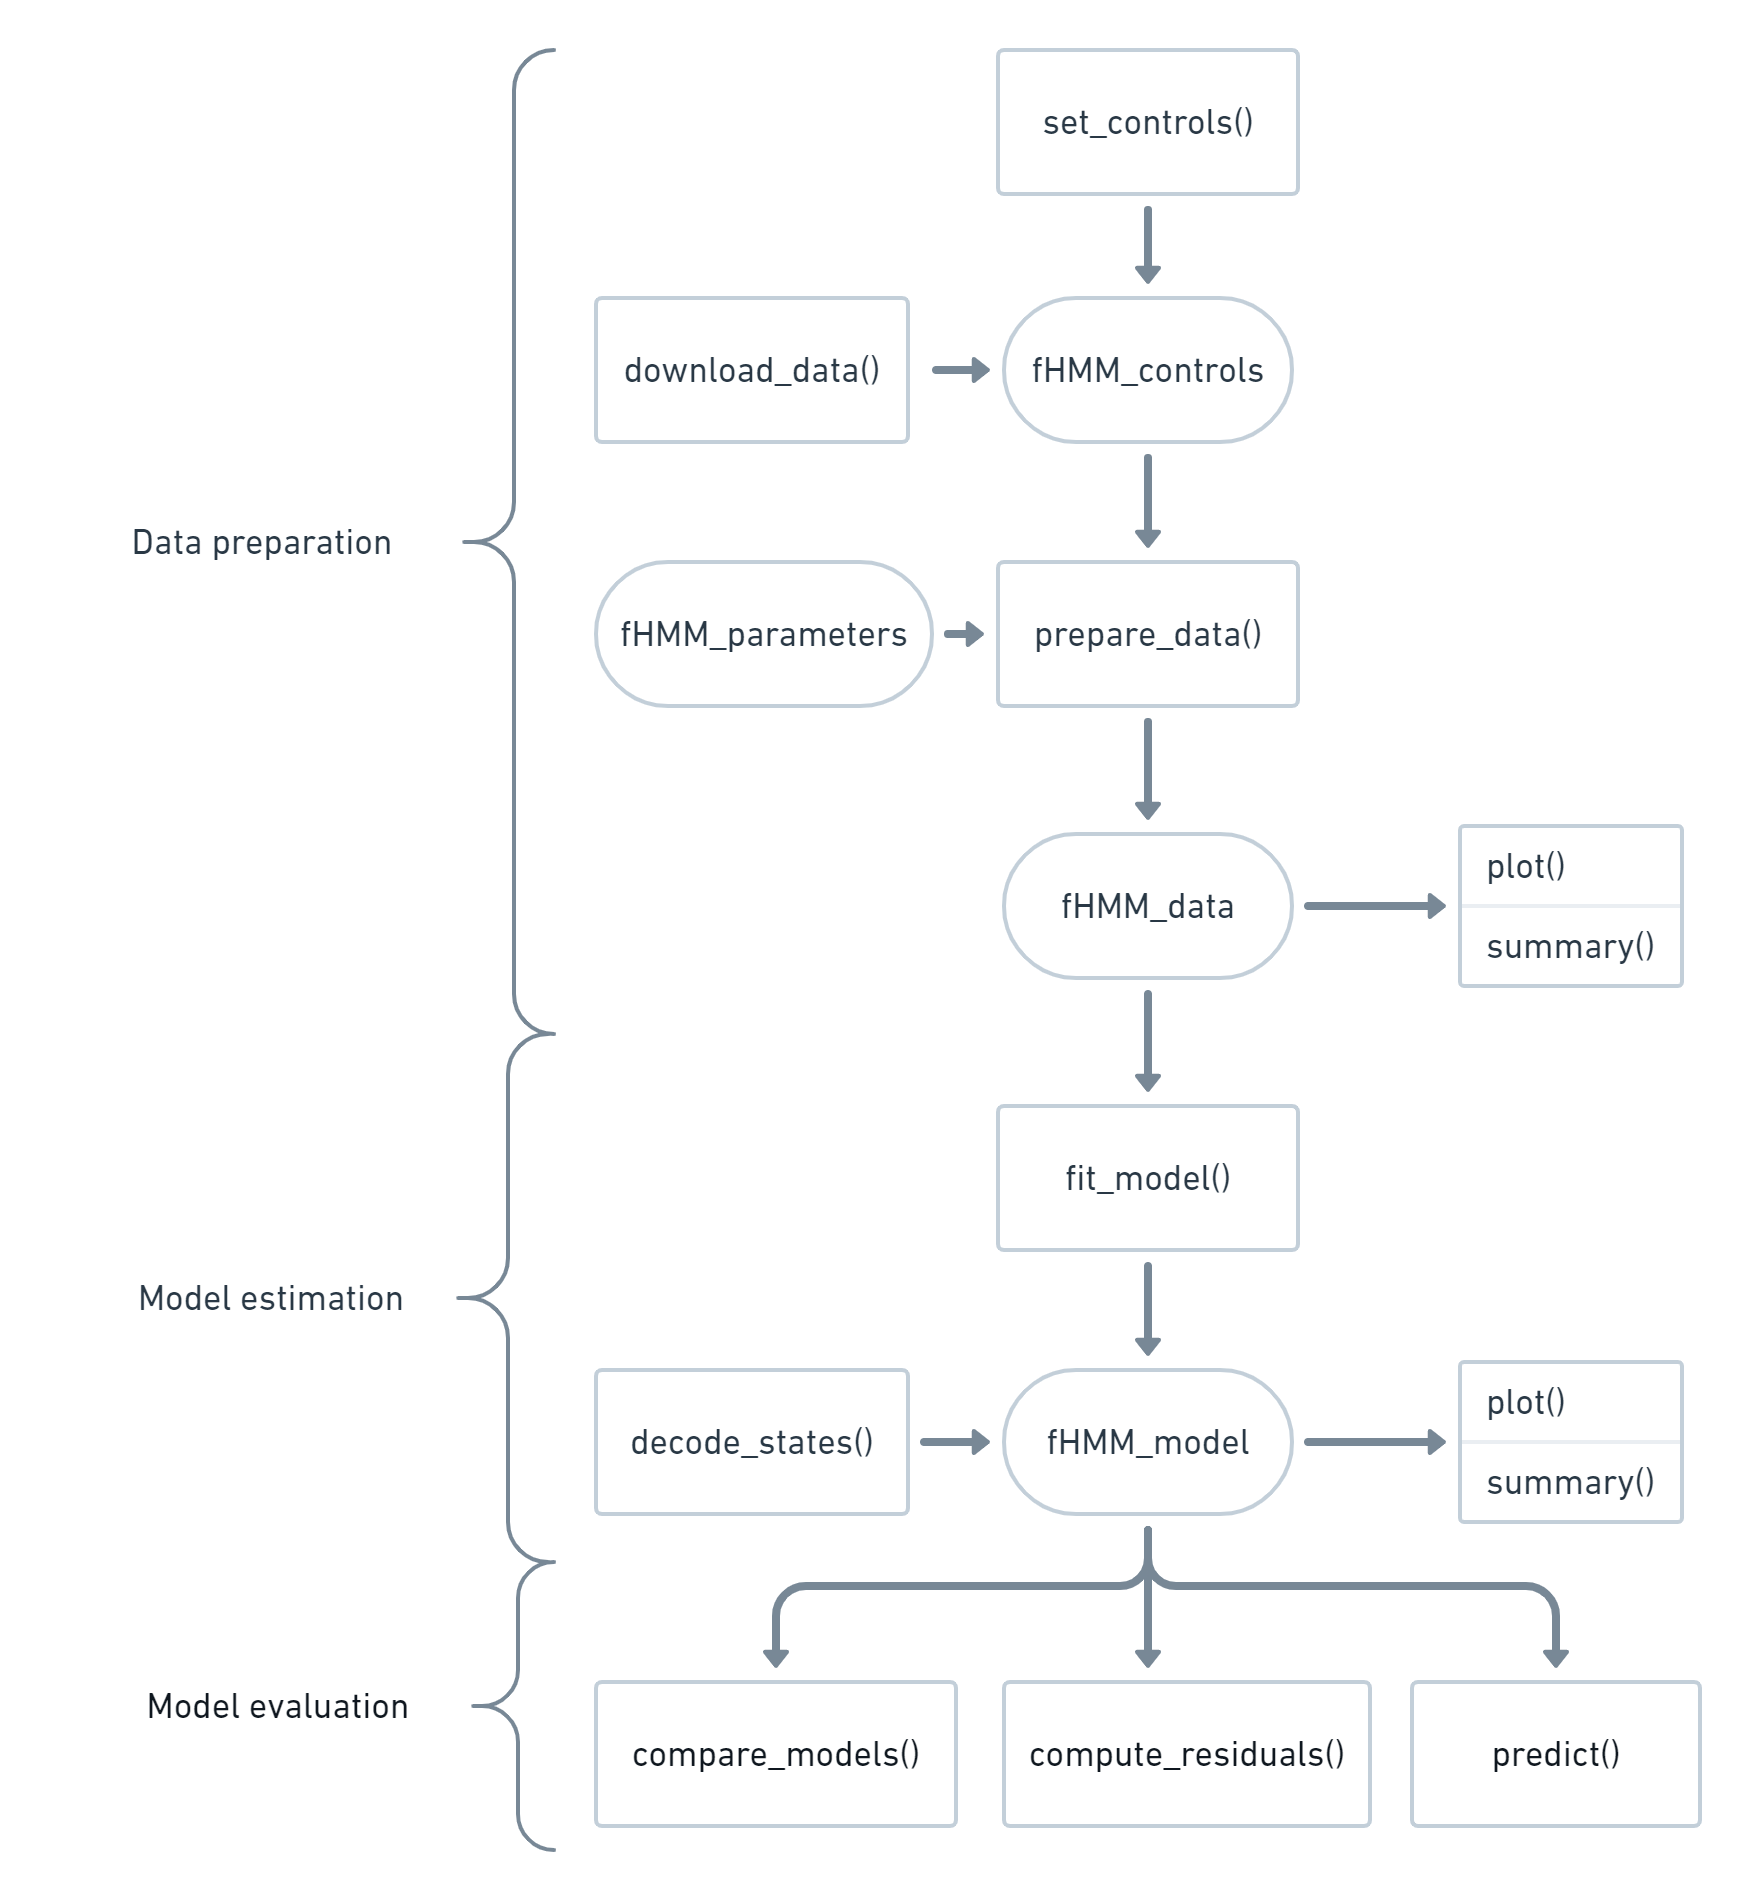
\includegraphics[scale = 0.5]{flowchart.png}
  \caption{Flowchart of the package functionality.}
  \label{fig:flowchart}
\end{figure}

%% Outline of the paper
This paper is structured as follows: in Section 2, ... In Section 3, ...

%% -- Manuscript ---------------------------------------------------------------

%% - In principle "as usual" again.
%% - When using equations (e.g., {equation}, {eqnarray}, {align}, etc.
%%   avoid empty lines before and after the equation (which would signal a new
%%   paragraph.
%% - When describing longer chunks of code that are _not_ meant for execution
%%   (e.g., a function synopsis or list of arguments), the environment {Code}
%%   is recommended. Alternatively, a plain {verbatim} can also be used.
%%   (For executed code see the next section.)
%% - Tables are placed at the top of the page
%%   (\verb|[t!]|), centered (\verb|\centering|), with a caption below the table,
%%   column headers and captions in sentence style, and if possible avoiding
%%   vertical lines.
%% - Virtually all JSS manuscripts list source code along with the generated
%%   output. The style files provide dedicated environments for this.
%% - In R, the environments {Sinput} and {Soutput} - as produced by Sweave() or
%%   or knitr using the render_sweave() hook - are used (without the need to
%%   load Sweave.sty).
%% - Equivalently, {CodeInput} and {CodeOutput} can be used.
%% - The code input should use "the usual" command prompt in the respective
%%   software system.
%% - For R code, the prompt "R> " should be used with "+  " as the
%%   continuation prompt.
%% - Comments within the code chunks should be avoided - these should be made
%%   within the regular LaTeX text.
%% - Please make sure that all code is properly spaced, e.g., using
%%   \code{y = a + b * x} and \emph{not} \code{y=a+b*x}.
%% - JSS prefers when the second line of code is indented by two spaces.

\section{Model definition} \label{sec:model_definition} %% Rouven

Hidden Markov models (HMMs) are a modeling framework for time series data where a sequence of observation is assumed to depend on a latent state process. The peculiarity is that, instead of the observation process, the state process cannot be directly observed. However, the latent states comprise information about the environment the model is applied on. 

The connection between hidden state process and observed state-dependent process arises by the following: Let $N$ be the number of possible states. We assume that for each point in time $t = 1, \ldots, T$, an underlying process $(S_t)_{t = 1, \ldots, T}$ is in one of those $N$ states. Then, depending on the active state $S_t \in \{ 1, \ldots, N \}$, the observation $X_t$ from the state-dependent process $(X_t)_{t = 1, \ldots, T}$ is assumed to be generated by the corresponding distribution of the $N$ distributions $f^{(1)},\dots,f^{(N)}.$

Furthermore, we assume $(S_t)_t$ to be Markovian, i.e.\ we assume that the actual state only depends on the previous state. Henceforth, we can identify the process by its initial distribution $\delta$ and its transition probability matrix (t.p.m.) $\Gamma$. Moreover, by construction, we force the process $(X_t)_{t = 1, \ldots, T}$ to satisfy the conditional independence assumption, i.e.\ the actual observation $X_t$ depends on the current state $S_t$, but does not depend on previous observations or states at all.

Referring to financial data, the different states can serve as proxies for the actual market situation, e.g. calm or nervous. Even though these moods cannot be observed directly, price changes or trading volumes, which clearly depend on the current mood of the market, can be observed. Thereby, using an underlying Markov process, we can detect which mood is active at any point in time and how the different moods alternate. Depending on the current mood, a price change is generated by a different distribution. These distributions characterize the moods in terms of expected return and volatility. For example, we can model price changes at time point $t$ to be generated by different normal distributions whose mean and volatility depend on $S_t$.

Following \cite{zuc16}, we assume that the initial distribution $\delta$ equals the stationary distribution $\pi$, where $\pi = \pi \Gamma$, i.e.\ the stationary and henceforth the initial distribution is determined by $\Gamma$. If the Markov process is irreducible, it has a unique distribution, which solves $\pi = \pi \Gamma$. If
additionally the Markov process is aperiodic, its state distribution converges to the stationary distribution, see \cite{nor97}. Irreducibility and aperiodicity are usually satisfied assumptions in reality. This is reasonable from a practical point of view: On the one hand, the hidden state process has been evolving for some time before we start to observe it and hence can be assumed to be stationary. On the other hand, setting $\delta=\pi$ reduces the number of parameters that need to be estimated, which is convenient from a computational perspective.

The hierarchical hidden Markov model (HMMM) is a flexible extension of the HMM  that can jointly model data observed on two different time scales. The two time series, one on a coarser and one on a finer scale, differ in the number of observations, e.g. monthly observations on the coarser scale and daily or weekly observations on the finer scale. 

Following the concept of HMMs, we can model both state-dependent time series jointly. First, we treat the time series on the coarser scale as stemming from an ordinary HMM, which we refer to as the coarse-scale HMM: At each time point $t$ of the coarse-scale time space $\{1,\dots,T\}$, an underlying process $(S_t)_t$ selects one state from the coarse-scale state space $\{1,\dots,N\}$. We call $(S_t)_t$ the hidden coarse-scale state process. Depending on which state is active at $t$, one of $N$ distributions $f^{(1)},\dots,f^{(N)}$ realizes the observation $X_t$. The process $(X_t)_t$ is called the observed coarse-scale state-dependent process. The processes $(S_t)_t$ and $(X_t)_t$ have the same properties as before, namely $(S_t)_t$ is a first-order Markov process and $(X_t)_t$ satisfies the conditional independence assumption. 

Subsequently, we segment the observations of the fine-scale time series into $T$ distinct chunks, each of which contains all data points that correspond to the $t$-th coarse-scale time point. Assuming that we have $T^*$ fine-scale observations on every coarse-scale time point, we face $T$ chunks comprising of $T^*$ fine-scale observations each. 

The hierarchical structure now evinces itself as we model each of the chunks by one of $N$ possible fine-scale HMMs. Each of the fine-scale HMMs has its own t.p.m.\ $\Gamma^{*(i)}$, initial distribution $\delta^{*(i)}$, stationary distribution $\pi^{*(i)}$, and state-dependent distributions $f^{*(i,1)},\dots,f^{*(i,N^*)}$. Which fine-scale HMM is selected to explain the $t$-th chunk of fine-scale observations depends on the hidden coarse-scale state $S_t$. The $i$-th fine-scale HMM explaining the $t$-th chunk of fine-scale observations consists of the following two stochastic processes: At each time point $t^*$ of the fine-scale time space $\{1,\dots,T^*\}$, the process $(S^*_{t,t^*})_{t^*}$ selects one state from the fine-scale state space $\{1,\dots,N^*\}$. We call $(S^*_{t,t^*})_{t^*}$ the hidden fine-scale state process. Depending on which state is active at $t^*$, one of $N^*$ distributions $f^{*(i,1)},\dots,f^{*(i,N^*)}$ realizes the observation $X^*_{t,t^*}$. The process $(X^*_{t,t^*})_{t^*}$ is called the observed fine-scale state-dependent process. 

The fine-scale processes $(S^*_{1,t^*})_{t^*},\dots,(S^*_{T,t^*})_{t^*}$ and $(X^*_{1,t^*})_{t^*},\dots,(X^*_{T,t^*})_{t^*}$ satisfy the Markov property and the conditional independence assumption, respectively, as well. Furthermore, it is assumed that the fine-scale HMM explaining $(X^*_{t,t^*})_{t^*}$ only depends on $S_t$. This hierarchical structure is visualized in Figure \ref{fig:hhmm}.

\begin{figure}
  \centering
  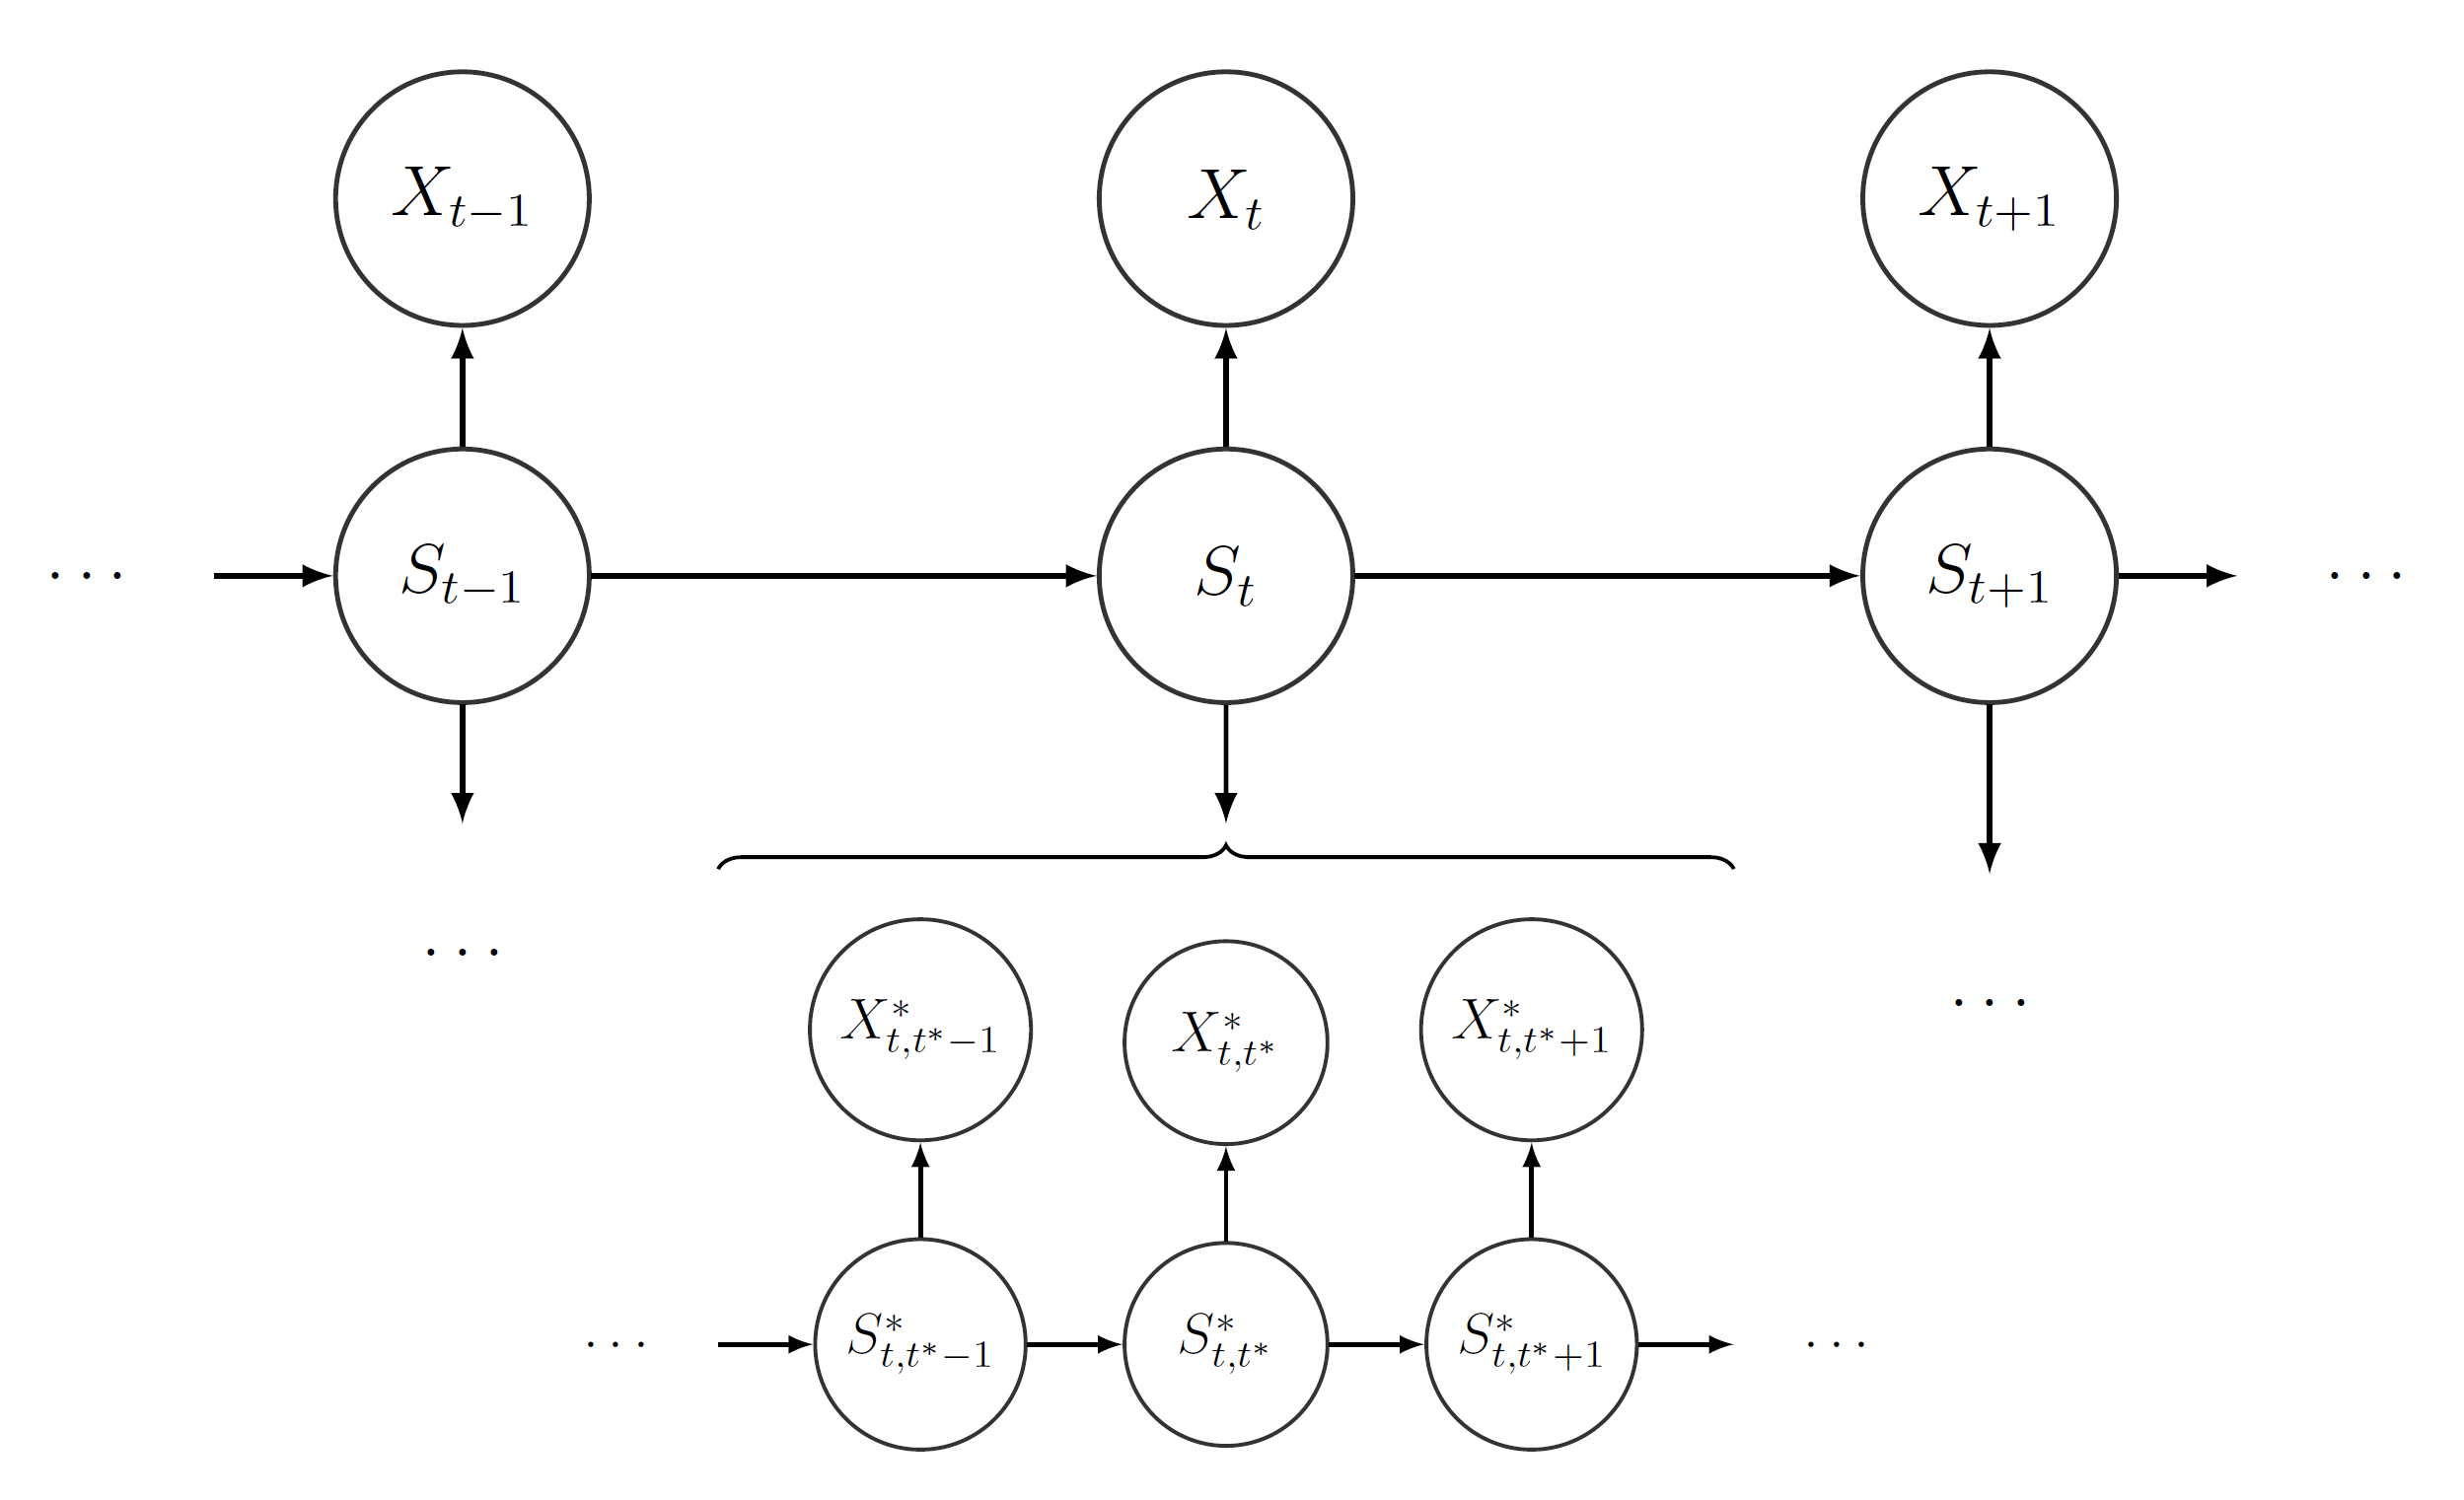
\includegraphics[scale = 0.5]{hhmm.png}
  \caption{Dependence structure of an HHMM.}
  \label{fig:hhmm}
\end{figure}

\section{Controls} \label{sec:controls} %% Lennart

The \pkg{fHMM} philosophy is to start the modeling process by setting all data, model, and estimation specifications. This is done by defining a named list of controls and passing it to the \fct{set\_controls} function. The function checks the specifications and returns an \class{fHMM\_controls} object which stores all specifications and thereby provides required information for other \pkg{fHMM} functionalities.

For demonstration, we list example specifications using data from the Deutscher Aktienindex DAX \cite{jan92}:

%
\begin{Schunk}
\begin{Sinput}
R> download_data(symbol = "^GDAXI", file = "dax.csv")
\end{Sinput}
\begin{Soutput}
Download successful.
* symbol: ^GDAXI 
* from: 1987-12-30 
* to: 2022-04-04 
* path: C:\Users\rouve\Documents\R\fHMM\fHMM\jss\dax.csv
\end{Soutput}
\end{Schunk}
%

The following lines of code specify a 3-state HMM with state-dependent t-distributions on the data in the file dax.csv. The dates are provided in the column called Date and the data in the column called Close. The \code{logreturns = TRUE} line transforms the index data to log-returns. The \code{runs = 50} line sets the number of numerical optimization runs to 50.

%
\begin{Schunk}
\begin{Sinput}
R> controls = list(
+    states = 3,
+    sdds   = "t",
+    data   = list(file        = "dax.csv",
+                  date_column = "Date",
+                  data_column = "Close",
+                  logreturns  = TRUE),
+    fit    = list(runs        = 50)
+  )
R> set_controls(controls)
\end{Sinput}
\begin{Soutput}
fHMM controls:
* hierarchy: FALSE 
* data type: empirical 
* number of states: 3 
* sdds: t() 
* number of runs: 50  
\end{Soutput}
\end{Schunk}
%

The following specifies a 2-state HMM with state-dependent Gamma distributions, where the expectation values for state 1 and 2 are fixed to -1 and 1, respectively. The model will be fitted to 500 data points (\code{horizon = 500}), that are going to be simulated from this model specification.

%
\begin{Schunk}
\begin{Sinput}
R> controls = list(
+    states  = 2,
+    sdds    = "gamma(mu = -1|1)",
+    horizon = 500
+  )
R> set_controls(controls)
\end{Sinput}
\begin{Soutput}
fHMM controls:
* hierarchy: FALSE 
* data type: simulated 
* number of states: 2 
* sdds: gamma(mu = -1|1) 
* number of runs: 100  
\end{Soutput}
\end{Schunk}
%

Specifying hierarchical HMMs is analogously, except that new parameters can be specified (for example \code{period}, see below) and some parameters now can be specified for both hierarchies.

%
\begin{Schunk}
\begin{Sinput}
R> controls = list(
+    hierarchy = TRUE,
+    horizon   = c(100, 10),
+    sdds      = c("t(df = 1)", "t(df = Inf)"),
+    period    = "m"
+  )
R> set_controls(controls)
\end{Sinput}
\begin{Soutput}
fHMM controls:
* hierarchy: TRUE 
* data type: simulated 
* number of states: 2 2 
* sdds: t(df = 1) t(df = Inf) 
* number of runs: 100  
\end{Soutput}
\end{Schunk}
%

The help page of the \fct{set\_controls} function provides an overview of all possible specifications, see the appendix.

\section{Data management} \label{sec:data_management} %% Lennart

Empirical data must be provided as a comma-separated values (CSV) file and its path must be specified in \fct{set\_controls`}. The \fct{download\_data} function explained below provides a convenient tool for downloading stock data from https://www.yahoo.com/finance in csv-format. The \pkg{fHMM} package comes with two datasets of the Deutscher Aktienindex and the VW stock for demonstration purpose that can be accessed as follows:

%
\begin{Schunk}
\begin{Sinput}
R> system.file("extdata", "dax.csv", package = "fHMM")
\end{Sinput}
\begin{Soutput}
[1] ""
\end{Soutput}
\begin{Sinput}
R> system.file("extdata", "vw.csv", package = "fHMM")
\end{Sinput}
\begin{Soutput}
[1] ""
\end{Soutput}
\end{Schunk}
%

The \code{prepare\_data} function prepares the data based on the \class{data} controls specifications and returns an \class{fHMM\_data} object that can be passed to the \fct{fit\_model} function for model fitting.

%
\begin{Schunk}
\begin{Sinput}
R> controls <- list(
+    states = 3,
+    sdds   = "t",
+    data   = list(file        = system.file("extdata", "dax.csv", package = "fHMM"),
+                  date_column = "Date",
+                  data_column = "Close",
+                  logreturns  = TRUE)
+  )
R> controls <- set_controls(controls)